\subsection{Analog-to-Digital Converter (ADC)}


\begin{figure}[H]
	\centering
	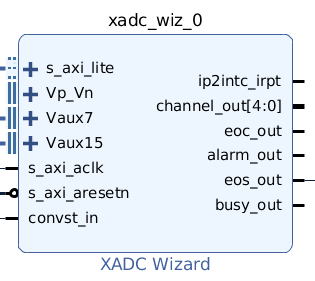
\includegraphics[width=0.45\textwidth]{pictures/software/adc.png}
	\caption{}
	\label{fig:adc_module}
\end{figure}



\begin{figure}[H]
	\centering
	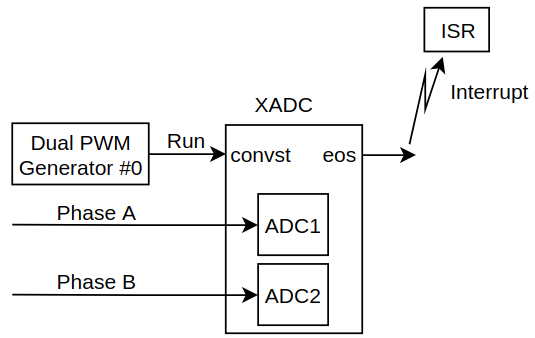
\includegraphics[width=0.6\textwidth]{pictures/software/adc_block_diagram.png}
	\caption{}
	\label{fig:adc_block_diagram}
\end{figure}


 Due to the symmetry between the three phases only two of the phases needs to be calculated. The third phase can be calculated from equation \ref{eq:third_phase}.
\begin{equation}
    I_C = -(I_A + I_B)
    \label{eq:third_phase}
\end{equation}

The calculation of the last phase is done in the processing system.
